\documentclass[10pt, compress,usetitleprogressbar,aspectratio=1610]{beamer}

\usetheme{m}
\usepackage[scale=2]{ccicons}
\usepackage{minted}
\usepackage{hyperref}
\usepackage{multicol}
\usepackage{multirow}
\usepackage[official]{eurosym}

\usemintedstyle{trac}

% Presentation theme: https://github.com/matze/mtheme
% Requirements:
% - Xelatex
% - Fira fonts (http://www.carrois.com/fira-4-0/#download, install Sans and Mono)
% - Pygments (sudo pip install pygments, if pip is not installed do sudo apt-get install python-pip)
% - The Makefile takes care of the compilation options. Make continuous adds the -pvc option for continuous preview

\hypersetup{
  hyperindex,
    colorlinks,
    allcolors=blue!60!black
}

\title{Fault Manager Lite}
\subtitle{Project plan - Goals, estimations and planning}
\date{\today}
\author{Iván Márquez Pardo \and Víctor de Juan Sanz \and Guillermo Julián Moreno}
\institute{Triforce}

\begin{document}

\maketitle

\begin{frame}
\frametitle{Contents}
\tableofcontents
\end{frame}

\section{Introduction}
\begin{frame}[fragile]
\frametitle{Project definition}

Fault Manager Lite is the future system that will fulfill the necessities of the UAM regarding notification and management of faults that arise on campus.

FML unifies a fault report system with a task manager with the aim of speeding up fault troubleshooting. Users will be able to report faults in \emph{less than two minutes}. Technicians will automatically be assigned on them based on their location and department.
\end{frame}

\section{Project definition}

\begin{frame}
\frametitle{Goals}

\begin{itemize}
\item \textbf{Reduce fault detection time} in order to facilitate a quick troubleshooting.
\item \textbf{Efficient allocation of resources} relying on automatic systems and crowdsourced reports instead of manual management.
\item \textbf{Coordination} of all the maintenance staff.
\item \textbf{Facilitate reports} in a way that users can communicate what's wrong without spending too much time.
\end{itemize}
\end{frame}

\begin{frame}
\frametitle{Subsystems \hfill \emph{II}}
\begin{itemize}
\item \alert{Task management} Responsible for receiving and analyzing reports. Aspects like task assignments, priority categorization and repair status will be managed by this subsystem.
\item \alert{Reporting} Will allow users to send reports about discovered faults. It will also detect duplicates before sending them to the task manager.
\item \alert{Notification \& messaging} Responsible for notifying technicians and users about emergencies, changes and updates in reports. It will also allow private communication channels between reporters and technicians.
\end{itemize}
\end{frame}

\begin{frame}
\frametitle{Subsystems \hfill \emph{II}}
\begin{itemize}
\item \alert{User management} Communicates with the UAM login server in order to authenticate users. Keeps a profile on each user who registered within the system, their role and their fault report history.
\item \alert{Fault history \& stats} Tracks changes in the fault reports and generates statistics based on them, either for the whole system, for each department or even for a specific user of the system. It will also allow visualization of all the reported faults in a campus map.
\end{itemize}
\end{frame}

\section{Project estimation}

\subsection{Size estimation}
\begin{frame}
\frametitle{Size estimation \hfill \emph{Function points - Whole system}}
\begin{table}[hbtp]
\centering

\begin{tabular}{|l|c|c|c|c|c|c|c|}
\cline{2-7}
\multicolumn{1}{c}{} & \multicolumn{6}{|c|}{\textsc{Complexity}} & \multicolumn{1}{c}{}  \\ \cline{2-8}
\multicolumn{1}{c|}{} & \textbf{Low} & \textbf{Medium} & \textbf{High} & \textbf{Low} & \textbf{Medium} & \textbf{High} & \multirow{2}{*}{\textit{Unadjusted FP}} \\ \cline{1-7}
\textbf{Data fns.} & \multicolumn{3}{|c|}{\textit{Frequency}} &  \multicolumn{3}{|c|}{\textit{Weight}} & \\ \hline
ILF 	& 15 & 1 & 0 & 7 & 10 & 15 & 115 	\\ \hline
EIF 	& 1  & 0 & 0 & 5 & 7 & 10 & 5		\\ \hline
\textbf{Transactional fns.} & \multicolumn{7}{|c|}{} \\ \hline
EI 		& 2  & 0 & 0 & 3 & 4 & 6 & 6 		\\ \hline
EO 		& 0  & 3 & 0 & 4 & 5 & 7 & 15		\\ \hline
EQ		& 15 & 0 & 0 & 3 & 4 & 6 & 45		\\ \hline
\multicolumn{6}{c|}{} & \textbf{Total} & 186.0 \\ \cline{7-8}
\end{tabular}

\caption{Detailed breakdown of the estimation of the project size in terms of function points.}
\label{tblFunctionPointsSize}
\end{table}
\end{frame}

\begin{frame}
\frametitle{Size estimation \hfill \emph{Function points - Subsystem breakdown}}
\begin{table}[hbtp]
\centering

\begin{tabular}{l|c|c}
\textbf{Subsystem} & \textbf{UFP} & \textbf{AFP} \\ \hline
Task Management	& 93.0 & 102.3 \\
Report System & 13.0 & 14.3 \\
Notification and Messaging System & 16.0 & 17.6 \\
User Management & 28.0 & 30.8 \\
Faults History and Statistics & 33.0 & 36.3 \\ \hline
\textit{Total} & \textit{183.0} & \textit{201.3}
\end{tabular}
\caption{Breakdown of unadjusted (UFP) and adjusted (AFP) function points for each subsystem.}
\end{table}
\end{frame}

% % % % % % % % % % % % % Start of subsystem's size estimation % % % % % % % % % % % %



\begin{frame}
\frametitle{Size estimation \hfill \emph{Function points - Task Management}}
\begin{table}[hbtp]
\centering

\begin{tabular}{|l|c|c|c|c|c|c|c|}
\cline{2-7}
\multicolumn{1}{c}{} & \multicolumn{6}{|c|}{\textsc{Complexity}} & \multicolumn{1}{c}{}  \\ \cline{2-8}
\multicolumn{1}{c|}{} & \textbf{Low} & \textbf{Medium} & \textbf{High} & \textbf{Low} & \textbf{Medium} & \textbf{High} & \multirow{2}{*}{\textit{Unadjusted FP}} \\ \cline{1-7}
\textbf{Data fns.} & \multicolumn{3}{|c|}{\textit{Frequency}} &  \multicolumn{3}{|c|}{\textit{Weight}} & \\ \hline
ILF 	& 11 & 0 & 0 & 7 & 10 & 15 & 77 	\\ \hline
EIF 	& 0 & 0 & 0 & 5 & 7 & 10 & 0		\\ \hline
\textbf{Transactional fns.} & \multicolumn{7}{|c|}{} \\ \hline
EI 		& 0 & 0 & 0 & 3 & 4 & 6 & 0 		\\ \hline
EO 		& 0 & 0 & 0 & 4 & 5 & 7 & 0		\\ \hline
EQ		& 3 & 0 & 0 & 3 & 4 & 6 & 9		\\ \hline
\multicolumn{6}{c|}{} & \textbf{Total} & 86.0 \\ \cline{7-8}
\end{tabular}

\caption{Detailed breakdown of the estimation of the subsystem size in terms of function points.}
\label{tblFunctionPointsSize}
\end{table}
\end{frame}

\begin{frame}
\frametitle{Size estimation \hfill \emph{Function points - Report System}}
\begin{table}[hbtp]
\centering

\begin{tabular}{|l|c|c|c|c|c|c|c|}
\cline{2-7}
\multicolumn{1}{c}{} & \multicolumn{6}{|c|}{\textsc{Complexity}} & \multicolumn{1}{c}{}  \\ \cline{2-8}
\multicolumn{1}{c|}{} & \textbf{Low} & \textbf{Medium} & \textbf{High} & \textbf{Low} & \textbf{Medium} & \textbf{High} & \multirow{2}{*}{\textit{Unadjusted FP}} \\ \cline{1-7}
\textbf{Data fns.} & \multicolumn{3}{|c|}{\textit{Frequency}} &  \multicolumn{3}{|c|}{\textit{Weight}} & \\ \hline
ILF 	& 1 & 0 & 0 & 7 & 10 & 15 & 7 	\\ \hline
EIF 	& 0 & 0 & 0 & 5 & 7 & 10 & 0		\\ \hline
\textbf{Transactional fns.} & \multicolumn{7}{|c|}{} \\ \hline
EI 		& 2 & 0 & 0 & 3 & 4 & 6 & 6		\\ \hline
EO 		& 0 & 0 & 0 & 4 & 5 & 7 & 0		\\ \hline
EQ		& 0 & 0 & 0 & 3 & 4 & 6 & 0		\\ \hline
\multicolumn{6}{c|}{} & \textbf{Total} & 13.0 \\ \cline{7-8}
\end{tabular}

\caption{Detailed breakdown of the estimation of the subsystem size in terms of function points.}
\label{tblFunctionPointsSize}
\end{table}
\end{frame}

\begin{frame}
\frametitle{Size estimation \hfill \emph{Function points - Notification and Messaging system}}
\begin{table}[hbtp]
\centering

\begin{tabular}{|l|c|c|c|c|c|c|c|}
\cline{2-7}
\multicolumn{1}{c}{} & \multicolumn{6}{|c|}{\textsc{Complexity}} & \multicolumn{1}{c}{}  \\ \cline{2-8}
\multicolumn{1}{c|}{} & \textbf{Low} & \textbf{Medium} & \textbf{High} & \textbf{Low} & \textbf{Medium} & \textbf{High} & \multirow{2}{*}{\textit{Unadjusted FP}} \\ \cline{1-7}
\textbf{Data fns.} & \multicolumn{3}{|c|}{\textit{Frequency}} &  \multicolumn{3}{|c|}{\textit{Weight}} & \\ \hline
ILF 	& 1 & 0 & 0 & 7 & 10 & 15 & 7 	\\ \hline
EIF 	& 0 & 0 & 0 & 5 & 7 & 10 & 0		\\ \hline
\textbf{Transactional fns.} & \multicolumn{7}{|c|}{} \\ \hline
EI 		& 0 & 0 & 0 & 3 & 4 & 6 & 0 		\\ \hline
EO 		& 0 & 0 & 0 & 4 & 5 & 7 & 0		\\ \hline
EQ		& 3 & 0 & 0 & 3 & 4 & 6 & 9		\\ \hline
\multicolumn{6}{c|}{} & \textbf{Total} & 16.0 \\ \cline{7-8}
\end{tabular}

\caption{Detailed breakdown of the estimation of the subsystem size in terms of function points.}
\label{tblFunctionPointsSize}
\end{table}
\end{frame}

\begin{frame}
\frametitle{Size estimation \hfill \emph{Function points - User Management}}
\begin{table}[hbtp]
\centering

\begin{tabular}{|l|c|c|c|c|c|c|c|}
\cline{2-7}
\multicolumn{1}{c}{} & \multicolumn{6}{|c|}{\textsc{Complexity}} & \multicolumn{1}{c}{}  \\ \cline{2-8}
\multicolumn{1}{c|}{} & \textbf{Low} & \textbf{Medium} & \textbf{High} & \textbf{Low} & \textbf{Medium} & \textbf{High} & \multirow{2}{*}{\textit{Unadjusted FP}} \\ \cline{1-7}
\textbf{Data fns.} & \multicolumn{3}{|c|}{\textit{Frequency}} &  \multicolumn{3}{|c|}{\textit{Weight}} & \\ \hline
ILF 	& 2 & 0 & 0 & 7 & 10 & 15 & 14 	\\ \hline
EIF 	& 1 & 0 & 0 & 5 & 7 & 10 & 5		\\ \hline
\textbf{Transactional fns.} & \multicolumn{7}{|c|}{} \\ \hline
EI 		& 0 & 0 & 0 & 3 & 4 & 6 & 0 		\\ \hline
EO 		& 0 & 0 & 0 & 4 & 5 & 7 & 0		\\ \hline
EQ		& 3 & 0 & 0 & 3 & 4 & 6 & 9		\\ \hline
\multicolumn{6}{c|}{} & \textbf{Total} & 28.0 \\ \cline{7-8}
\end{tabular}

\caption{Detailed breakdown of the estimation of the project size in terms of function points.}
\label{tblFunctionPointsSize}
\end{table}
\end{frame}

\begin{frame}
\frametitle{Size estimation \hfill \emph{Function points - Faults History and Statistics}}
\begin{table}[hbtp]
\centering

\begin{tabular}{|l|c|c|c|c|c|c|c|}
\cline{2-7}
\multicolumn{1}{c}{} & \multicolumn{6}{|c|}{\textsc{Complexity}} & \multicolumn{1}{c}{}  \\ \cline{2-8}
\multicolumn{1}{c|}{} & \textbf{Low} & \textbf{Medium} & \textbf{High} & \textbf{Low} & \textbf{Medium} & \textbf{High} & \multirow{2}{*}{\textit{Unadjusted FP}} \\ \cline{1-7}
\textbf{Data fns.} & \multicolumn{3}{|c|}{\textit{Frequency}} &  \multicolumn{3}{|c|}{\textit{Weight}} & \\ \hline
ILF 	& 0 & 0 & 0 & 7 & 10 & 15 & 0 	\\ \hline
EIF 	& 0 & 0 & 0 & 5 & 7 & 10 & 0		\\ \hline
\textbf{Transactional fns.} & \multicolumn{7}{|c|}{} \\ \hline
EI 		& 0 & 0 & 0 & 3 & 4 & 6 & 0 		\\ \hline
EO 		& 0 & 3 & 0 & 4 & 5 & 7 & 15		\\ \hline
EQ		& 6 & 0 & 0 & 3 & 4 & 6 & 18		\\ \hline
\multicolumn{6}{c|}{} & \textbf{Total} & 33.0 \\ \cline{7-8}
\end{tabular}

\caption{Detailed breakdown of the estimation of the project size in terms of function points.}
\label{tblFunctionPointsSize}
\end{table}
\end{frame}




% % % % % % % % % % % % % End of subsystem's size estimation % % % % % % % % % % % %



\subsection{Cost estimation}
\begin{frame}
\frametitle{Cost estimation \hfill \emph{COCOMO II for the Fault Report subsystem}}
A sample of the cost estimation, based on the most critical subsystem, the fault reporter. Necessary for a minimum prototype.

\begin{table}[hbtp]
\centering
\begin{tabular}{l|ccccc|c}
\multirow{2}{*}{\textbf{Phase}} & \textbf{Effort} & \textbf{Labour} & \textbf{Running} & \textbf{Fixed} & \textbf{Total} & \textbf{Duration} \\
& \textit{Person-months} & \textit{K\$} & \textit{K\$ / month} & \textit{K\$} & \textit{K\$} & \textit{Months} \\
\textsc{Requirements} & 0.1 & 0.8 & 1.05 & 0 & 1.535 & 0.7 \\
\textsc{Product design} & 0.3 & 1.5 & 1.05 & 0 & 2.55 & 1 \\
\textsc{Detailed design} & 0.4 & 2.3 & 1.05 & 0 & 3.35 & 1 \\
\textsc{Code \& Unit tests} & 0.5 & 2.8 & 1.05 & 8.25 & 12.415 & 1.3 \\
\textsc{Integration \& test} & 0.3 & 1.6 & 1.05 & 3.2 & 5.64 & 0.8 \\ \hline
\textsc{Development} & 1.5 & 8.2 & N/A & 11.45 & 23.955 & 4.1 \\
\textsc{Totals} & 1.6 & 9 & N/A & 11.45 & 25.49 & 4.8
\end{tabular}

\caption{Cocomo cost estimation for the fault report subsystem.}
\label{tblFaultReportCost}
\end{table}
\end{frame}

\section{Project planning}

\subsection{Effort estimations}
\begin{frame}
\frametitle{Time estimation \hfill \emph{Whole project}}
Given the size estimations and Triforce project data, this is the time estimation for the project.

\begin{table}[hbtp]
\centering
\begin{tabular}{l|c}
\textbf{Summary} & \textbf{Value} \\ \hline
Raw function points (FP) & 183 \\
Complexity factor (CF) & 45 \\
Adjustment factor & 1.10 \\
Adjusted function points & 201.3 \\
Person/day per function points & 1.466 \\ \hline
\textit{Estimated person-days} & \textit{295.1058}
\end{tabular}

\caption{Time estimation based on function points for the system (see table \ref{tblFunctionPointsSize}).}
\label{tblFunctionPointsTime}
\end{table}
\end{frame}


% % % % % % % % % % % % % Start of subsystem's time estimation % % % % % % % % % % % %


\begin{frame}
\frametitle{Size estimation \hfill \emph{Function points - Task Management}}
\begin{table}[hbtp]
\centering
\begin{tabular}{l|c}
\textbf{Summary} & \textbf{Value} \\ \hline
Raw function points (FP) & 93 \\
Complexity factor (CF) & 45 \\
Adjustment factor & 1.10 \\
Adjusted function points & 102.3 \\
Person/day per function points & 1.466 \\ \hline
\textit{Estimated person-days} & \textit{149.972}
\end{tabular}

\caption{Time estimation based on function points for the subsystem.}
\label{tblFunctionPointsSize}
\end{table}
\end{frame}


\begin{frame}
\frametitle{Size estimation \hfill \emph{Function points - Report System}}
\begin{table}[hbtp]
\centering
\begin{tabular}{l|c}
\textbf{Summary} & \textbf{Value} \\ \hline
Raw function points (FP) & 13 \\
Complexity factor (CF) & 45 \\
Adjustment factor & 1.10 \\
Adjusted function points & 14.3 \\
Person/day per function points & 1.615 \\ \hline
\textit{Estimated person-days} & \textit{23.0945}
\end{tabular}

\caption{Time estimation based on function points for the subsystem.}
\label{tblFunctionPointsSize}
\end{table}
\end{frame}


\begin{frame}
\frametitle{Size estimation \hfill \emph{Function points - Task Management}}
\begin{table}[hbtp]
\centering
\begin{tabular}{l|c}
\textbf{Summary} & \textbf{Value} \\ \hline
Raw function points (FP) & 16 \\
Complexity factor (CF) & 45 \\
Adjustment factor & 1.10 \\
Adjusted function points & 17.6 \\
Person/day per function points & 1.466 \\ \hline
\textit{Estimated person-days} & \textit{25.80}
\end{tabular}

\caption{Time estimation based on function points for the subsystem.}
\label{tblFunctionPointsSize}
\end{table}
\end{frame}


\begin{frame}
\frametitle{Size estimation \hfill \emph{Function points - User Management}}
\begin{table}[hbtp]
\centering
\begin{tabular}{l|c}
\textbf{Summary} & \textbf{Value} \\ \hline
Raw function points (FP) & 28 \\
Complexity factor (CF) & 45 \\
Adjustment factor & 1.10 \\
Adjusted function points & 30.8 \\
Person/day per function points & 1.615 \\ \hline
\textit{Estimated person-days} & \textit{49.742}
\end{tabular}

\caption{Time estimation based on function points for the subsystem.}
\label{tblFunctionPointsSize}
\end{table}
\end{frame}


\begin{frame}
\frametitle{Size estimation \hfill \emph{Function points - Faults History and Statistics}}
\begin{table}[hbtp]
\centering
\begin{tabular}{l|c}
\textbf{Summary} & \textbf{Value} \\ \hline
Raw function points (FP) & 33 \\
Complexity factor (CF) & 45 \\
Adjustment factor & 1.10 \\
Adjusted function points & 36.3 \\
Person/day per function points & 1.466 \\ \hline
\textit{Estimated person-days} & \textit{53.2158}
\end{tabular}

\caption{Time estimation based on function points for the subsystem.}
\label{tblFunctionPointsSize}
\end{table}
\end{frame}

% % % % % % % % % % % % % End of subsystem's time estimation % % % % % % % % % % % %


\subsection{Increment planning}
\begin{frame}
\frametitle{Increment planning}

Our schedule consists of 3 increments, detailed in the following table:

\begin{table}[hbtp]
\centering

\begin{tabular}{c|l|c|c}
\textbf{Increment} & \textbf{Subsystems} & \textbf{Function Points} & \textbf{Effort (person-days)} \\ \hline
Increment 1 & Task management & 102.3 & 149.972 \\
Increment 2 & Report System, Fault History & 50.6 & 74.213 \\
Increment 3 & Notification and Messaging & 48.4 & 70.986 \\ \hline
\textit{Total} &  & \textit{201.3} & \textit{295.106} \\
\end{tabular}

\caption{Planned increments for the development.}
\label{tblIncrements}
\end{table}
\end{frame}

\subsection{Schedule}
\begin{frame}
\frametitle{Schedule}
\begin{figure}[hbtp]
\centering
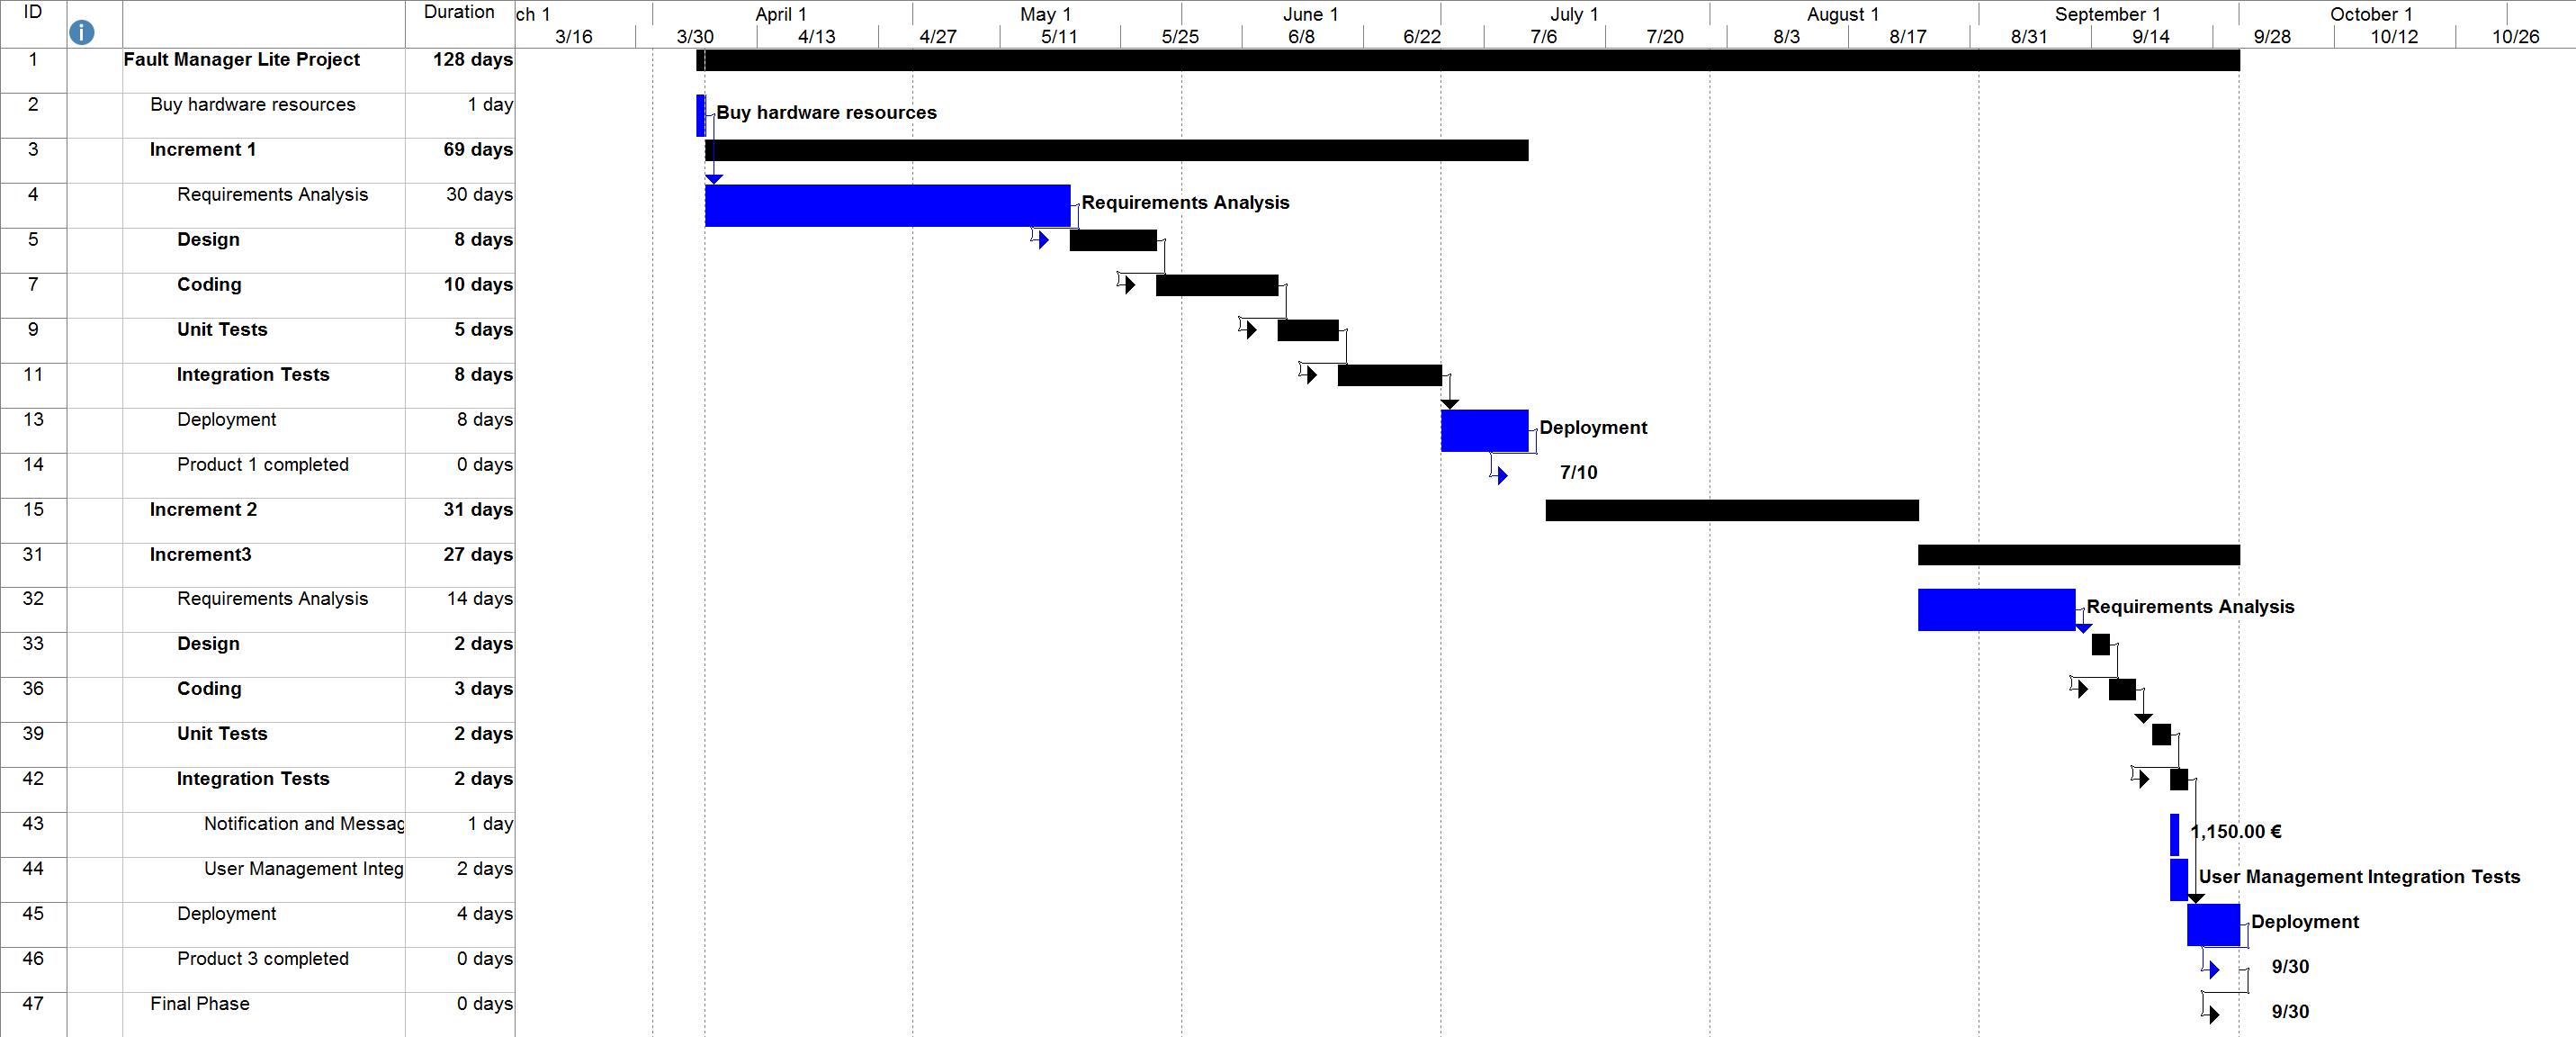
\includegraphics[width=\textwidth]{../GanttDiagram.png}
\caption{Proposed schedule as a Gantt diagram.}
\label{figGantt}
\end{figure}
\end{frame}

\subsection{Final cost estimation}
\begin{frame}
\frametitle{Final cost estimation}
\begin{table}[hbtp]
\centering
\begin{tabular}{r|lr|r}
\textbf{Resource} & \textbf{Quantity} & \textbf{Unit cost} & \textbf{Total cost} \\ \hline
System Analyst & 848 hours & 400 \euro / day & 42,400 \euro \\
Senior Designer & 504 hours & 350 \euro / day & 22,050 \euro \\
Junior Designer 1 & 504 hours & 200 \euro / day & 12,600 \euro \\
Junior Designer 2 & 504 hours & 200 \euro / day & 12,600 \euro \\
Systems Technician & 128 hours & 300 \euro / day & 4,800 \euro \\ \hline
\textit{Total work} & \textit{1,994 hours} & - & \textit{94,450 \euro} \\ \hline \hline
Systems Maintenance & 128 days & 1,050 \euro / month & 6,109 \euro \\
IDE Software & 3 workstations & 1,100 \euro / w.s. & 3,300 \euro \\
Development w.s. & 3 workstations & 1,650 \euro / w.s. & 4,950 \euro \\
Performance w.s. & 1 workstation & 3,200 \euro / w.s. & 3,200 \euro \\ \hline
\textit{Total systems} & - & - & \textit{17,559 \euro} \\ \hline \hline
\textit{Total cost} & - & - & \textit{112,009 \euro}

\end{tabular}

\caption{Final cost estimation for the proposed schedule.}
\label{tblCostEstimate}
\end{table}
\end{frame}

\section{Project control \& tracking procedure}

\begin{frame}
\frametitle{Progress monitorization}
At the end of each phase of each increment, the corresponding deliverables will be reviewed in a meeting hold by the responsible of the phase.

The team will be in permanent communication, so delays will be detected and corrected quickly. The schedule has been made in a way that small delays will be accommodated and won't affect the global times of the project.

If deemed necessary, a general meeting will decide on bigger delays that affect the whole project.
\end{frame}

\begin{frame}
\frametitle{Verification \& testing}
Standard Triforce practices apply. The project will be ready for CI (continuous integration): static code analysis, load and unit tests will be performed automatically. Source control system will enforce code reviews and adherence to the coding style.

The security and usability teams will review and evaluate the application to find issues and report them to the development team with the suggested corrections and/or mitigations.
\end{frame}

\section{Conclusions}

\begin{frame}
\frametitle{Conclusions}

\begin{itemize}
\item Fault Manager Lite will be able to fulfill the \textbf{required goals}: improve the fault reporting system and facilitate efficient allocation of resources in order to reduce fault detection and repair time.
\item A final version of the system can be finished in \textbf{128 days}.
\item Estimated cost for the whole project is \textbf{$\sim$ 110,000 \euro}.
\item \textbf{Project progress} will be tracked during meetings at each increment finalization.
\item The system will be thoroughly \textbf{tested} with unit tests, code analysis and review, performance tests and dedicated security and usability test teams.
\end{itemize}

\end{frame}

\plain{Questions?}

\end{document}
